% Chapter 3

\chapter{Background} % Main chapter title

\label{Chapter3} % For referencing the chapter elsewhere, use \ref{Chapter3} 

In this chapter, we start to present brief history of memory attacks and some
background information on control-flow attack in section
\ref{sec:control-flow-attack}. In section \ref{sec:remote-attestation}, we
discuss how remote attestation helps to detect control-flow attack. We present
ScaRR control flow model in section \ref{sec:scarr-model}. The chapter ends in
section \ref{sec:llvm}, which share an overview of LLVM that relevant to the
research. 

\section{Control Flow Attack}
\label{sec:control-flow-attack}

Control-flow attack happens when adversaries make a program to perform action of
their choice without statically modify the program binary but alter the runtime
properties of the program. The adversary intention can be to execute malicious
operations or to leak secret information. Many of this runtime software security
attacks are occured due to memory corruption bug in software written in
low-level languages like C and C++ \cite{szekeresSoKEternalWar2013}.

Once memory corruption is triggered, there are different exploit types which
adversary can use to perform the attack. Some of the relevant exploits are
control-flow hijack \cite{shachamGeometryInnocentFlesh2007,
schusterCounterfeitObjectorientedProgramming2015}  and data only attack
\cite{chenNonControlDataAttacksAre2005,
carliniControlFlowBendingEffectiveness2015}. 

Control-flow hijack can be classified further into code injection attack and
code reuse attack such as return oriented programming
\cite{roemerReturnorientedProgrammingSystems2012}.  Code injection attack will
inject code in the program which will execute action prepared by the attacker.
Code injection attack is already mitigated by solution like non-executable stack
(NX), Data Execution Prevention and \( W \bigoplus R \)
\cite{vanderveenMemoryErrorsPresent2012}. Code reuse attack will execute
malicous action without injecting any codes, hence can't be detected by
previosly mentioned defenses mechanism. As example, return-oriented program
chains together short instruction sequences already present in a program’s
address space, each of which ends in a \texttt{return} instruction.
Unfortunately, ROP can not be mitigated by \( W \bigoplus R \)
\cite{roemerReturnorientedProgrammingSystems2012}.

Memory error attacks and defenses have been always a continuous battle which
unfortunately has not shown that it is over. In 2016, Abera et al proposed to
use remote attestation to detect control flow attack
\cite{aberaCFLATControlFlowAttestation2016}. That paper opened many researches
in this area which we briefly presented in Chapter \ref{Chapter1}.
 
\section{Remote Attestation}
\label{sec:remote-attestation}

In this thesis we explore the use of remote attestation in detecting
control-flow attack. Remote attestation is the activity of making a claim about
properties of a remote target by supplying evidence to an appraiser over a
network \cite{cokerPrinciplesRemoteAttestation2011a}. The ubiquitous deployment
of IoT and different applications in the cloud require robust remote attestation
method to ensure detection when the application is attacked.  Remote attestation
scope was only covering static attestation of the application binary. However,
in the recent years there have been more sophisticated attack that can alter the
behavior of application so that static attestation does not suffice. 

In remote attestation, there are two roles involved, a trusted prover and a
verifier. A prover is the one that must prove that the software has not been
compromised. Verifier checks prover to ask the current state of runtime of the
program. Alternatively, prover also can just update verifier periodically
without being asked. The verifier compares the response from prover with the
local database which has been generated before. If any of measurement
mismatches, it means the has been violation due to an adversary's attack.

This research mainly focuses on offline measurement data generation for remote
attestation which is used by verifier to validate the control flow graph. In the
next section we discuss the detail of the control-flow model. We use LLVM in
implementing the offline program analyzer.

\section{ScaRR Control-Flow Model} 
\label{sec:scarr-model}

ScaRR \cite{toffaliniScaRRScalableRuntime2019} are taking lesson learned from
many former runtime remote attestation scheme to build model that can perform in
a scalable way and can perform remote attestation on complex system. ScaRR
control-flow model consists of two main components, checkpoint and list of
action. 

As many previous runtime attestation scheme, ScaRR models and validates the
attestion based on program's control flow graph. We need to run one-time
measurement computation to extract checkpoints and list of actions of the
program.

\subsection{Checkpoints} \label{sec:scarr-checkpoints} Checkpoint is basic block
of the program that delimit execution path of the program. ScaRR defines these
different checkpoint types:
\begin{itemize}
    \item Thread Beginning: demarcating the start of program/thread
    \item Thread End: demarcating the end of program/thread
    \item Exit Point: representing exit point from application such as system
    call or out of translation unit function/library call
    \item Virtual-Checkpoint: managing cases for loop or recursion
\end{itemize}

In a program there should be at least Thread Beginning and Thread End
checkpoints. Later depends on the structure of the program different checkpoint
is marked in the program CFG.

\subsection{List of Actions}

List of actions (LoA) are edges (marked by two checkpoints) that direct one
checkpoint to the next one. In program execution path, we only consider edges
that identify the unique execution path.

LoA is defined through the following notation:


$$[(BBL_{s1},BBL_{d1}),...,(BBL_{sn},BBL_{dn})]$$

Consider again the CFG in the Figure \ref{fig:simple-loop-checkpoints}. The LoA
between node 3 (Checkpoint Virtual) and node 10 (checkpoint ThreadEnd) is
$[(BBL_3, BBL_{10})]$. However, the LoA between node 0 and node 3 is $[]$ (empty
set).


\section{LLVM}
\label{sec:llvm}

LLVM is compiler framework that was developed by Chris Lattner which provides
portable program representation and different tooling. LLVM supports the
implementation of different frontend, backend and middle optimizer for various
programming languages \cite{lattnerLLVMCompilationFramework2004a}. 

\subsection{Intermediate Representation}

LLVM intermediate representation (IR) provides high-level information about
programs to support sophisticated analysis and transformations. However, the
representation is low-level enough to represent arbitrary programs and to allow
extensive optimization. As an example, consider a simple C program in listing
\ref{listing:sample-c}.

\begin{listing}[htbp]
    \inputminted[
    frame=lines,
    framesep=2mm,
    baselinestretch=1.2,
    fontsize=\footnotesize,
    linenos
    ]{c}{Code/03/sample.c}
    \caption{Simple C Program}    
    \label{listing:sample-c}
\end{listing}

The IR of the program can be seen in listing \ref{listing:sample-ll}. The text
representation below, is just one of form of IR. Beside this readable
instruction representation, LLVM IR also can be represented as byte code and in
memory representation. In the IR, each line contains LLVM instructions.
Instructions are grouped in basic blocks: container for instructions that
execute sequentially. This arrangement, makes application control flow graph
(CFG) to be explicit in the IR. The details of LLVM IR is available in the
Language Reference \cite{LLVMLanguageReferencea}.

\begin{listing}[htbp]
    \inputminted[
    frame=lines,
    framesep=2mm,
    baselinestretch=1.2,
    fontsize=\footnotesize,
    linenos
    ]{llvm}{Code/03/sample.ll}
    \caption{LLVM IR The Sample C Program}    
    \label{listing:sample-ll}
\end{listing}


\begin{figure}[htbp]
\centerline{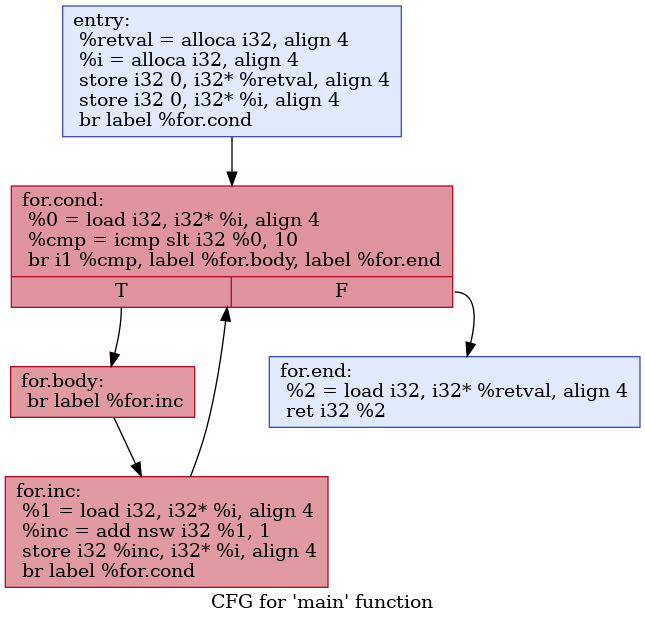
\includegraphics[scale=.5]{Figures/03/cfg.png}}
\caption{CFG for Simple C Program}
\label{fig:cfg}
\end{figure}


LLVM optimizer \textemdash{} which includes Analyzer and Transformer \textemdash{} are working on IR. In this thesis we are using this analyzer and transformer in building the Offline Program Analyzer.

\begin{figure}[htbp] 
    \centerline{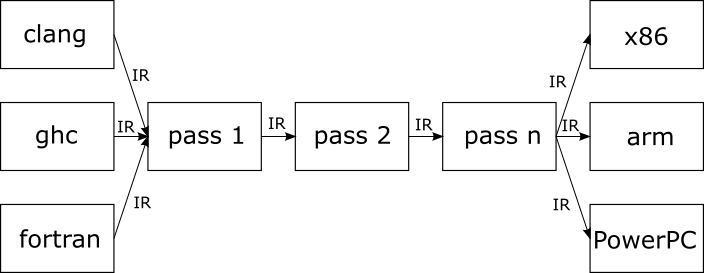
\includegraphics[scale=.75]{Figures/03/llvm-overview.png}} 
    \caption{LLVM Pass} 
    \label{fig:llvm} 
\end{figure} 

\subsection{LLVM Pass}

LLVM are applying transformations \textemdash{} which may include some analysis
pipelines \textemdash{} and optimizations on tools called \texttt{opt}.
\texttt{opt} is taking LLVM IR (either as text, bytecode or in memory) as input
and then do transformations, analysis and optimizations on it (see figure
\ref{fig:llvm}). Transformation and optimization alters the LLVM structure.
Analysis gets information from the structure, which usually to be used by one or
more transformations. Different transformations, optimizations and analyses are
performed as pipelines of LLVM passes. LLVM pass can run per function, module or
loop. LLVM function pass is executed once for every function in the program.
LLVM module pass is executed once for every module. LLVM loop pass runs a time
for each loop.  


In LLVM there are two ways of implementing Pass. First is using legacy approach
and the latest one is using new pass manager approach. The approach different in
structuring the code the implement the pass and also the way we use the pass.
In the legacy approach, we need to inherit from either \texttt{ModulePass},
\texttt{FunctionPass} or \texttt{LoopPass} and override \texttt{runOnXXX} method
(xxx is either Function, Module or Loop). In the newer approach we have to
inherit CRTP mix-in \texttt{PassInfoMixin<PassT>} and override the run method.

The way we use the pass, in legacy approach we need to provide the pass name as
literal argument to \texttt{opt}. See the example in listing
\ref{listing:legacy-llvm-pass}. In the new pass manager, we are putting the pass
name after `--passes` argument in comma separated list (listing
\ref{listing:new-llvm-pass}). The pass is executed in order.

\begin{listing}[htbp]
    \begin{minted}[
        frame=lines,
        framesep=2mm,
        baselinestretch=1.2,
        fontsize=\footnotesize,
        ]{bash}
        opt --dot-cfg file.ll 
    \end{minted}
    \caption{Running Legacy LLVM Pass}    
    \label{listing:legacy-llvm-pass}
\end{listing}

\begin{listing}[htpb]
    \begin{minted}[
        frame=lines,
        framesep=2mm,
        baselinestretch=1.2,
        fontsize=\footnotesize,
        ]{bash}
        opt -passes=scarr-cp-marker,scarr-loa-collector file.ll 
    \end{minted}
\caption{Running LLVM New Pass}    
\label{listing:new-llvm-pass}
\end{listing}

\subsection{LLVM API}

In writing LLVM pass, we use LLVM API. In this section we present relevant
component that is required in implementing LLVM Pass for the Offline Program
Analyzer. LLVM API is leveraging many C++ features and libraries such as
template and STL. The API also provides many ready to use data structure which
is not available in the STL. A more broad discussion on the important element of
the API is available in the Programmers Manual \cite{LLVMProgrammerManuala}.
Complete API documentation can be referred at the doxygen page \cite{LLVMLLVMa}.

\subsubsection{Module}

Module is the top level container for all other IR objects. Module contains list
of global variables, functions, symbol tables and other various data about
target characteristics. Module can be a single translation unit of a program
(source file) or can be multiple translation unit combined by linker. 

In LLVM pass, we can get access to module by implementing a Module pass or by
parsing IR using \texttt{parseIR} or \texttt{parseIRFile} from
\texttt{IRReader.h}. Once we get a handler to a module, getting a functions
within module is as simple as passing module to a loop, since module provides
iterator that return list of function in the module (see listing
\ref{listing:llvm-module-api}).

\begin{listing}[htbp]
    \inputminted[
        frame=lines,
        framesep=2mm,
        baselinestretch=1.2,
        fontsize=\footnotesize,
        linenos
    ]{cpp}{Code/03/module.cpp}
    \caption{LLVM Module API}    
    \label{listing:llvm-module-api}
\end{listing}

\subsubsection{Function}

Function in LLVM represents function in the source program. A function contains
list of zero or more BasicBlocks. There is one entry BasicBlock and can be
multiple exit BasicBlocks. We can get handler to a function either by getting
the iterator from a module instance or by implement a Function Pass. By using
optimization, syntax hint or using an inliner pass, a function can be inlined.
In this thesis, we are using \emph{inliner-wrapper} pass to inline most function
before feeding the IR into the ScaRR passes.

\subsubsection{Basic Block}

Basic Block represents single entry and single exit section of the code. The
single exit can be one of terminator instruction — branches, return, unwind and
invoke. We can get handle to a basic block from function. Refer to listing
\ref{listing:llvm-basic-block-api} to see how to get the basic block.

\begin{listing}[htbp]
    \begin{minted}[
        frame=lines,
        framesep=2mm,
        baselinestretch=1.2,
        fontsize=\footnotesize,
        linenos
    ]{cpp}
        for (auto &function: *module) {
            for (auto &basicBlok: function) {
                // do thing with Basic Block
            }
        }
    \end{minted}
    \caption{LLVM Basic Block API}    
    \label{listing:llvm-basic-block-api}
\end{listing}

\subsubsection{Graph Traversal}

Since LLVM CFG is already structured as a graph, the basic block can be
traversed using different ready to use graph traversal algorithm. LLVM offers
some common graph traversal algorithms such as breadth first search and depth
first search. The algorithms can be used immediately on basic blocks and
functions. If there is a need to traverse a custom structure, the algorithms
just require the new structure to implement \emph{GraphWriter} interface.

\subsection{Tools}

We are implementing the algorithms using different tools. We are highlighting
some of those in this section so that everyone interested can replicate the
step.

\subsubsection{clang}

\texttt{clang} is one of the frontend provided by LLVM. It can compiles C, C++
and Objective C. \texttt{clang} command line arguments are compatible with
widely use gcc compiler. The main use of \texttt{clang} in this research is to
compile source files into LLVM IR text files. Listing
\ref{listing:compile-llvm-to-ir} shows how to compile a C program into LLVM IR. 

\begin{listing}[htbp]
    \begin{minted}[
        frame=lines,
        framesep=2mm,
        baselinestretch=1.2,
        fontsize=\footnotesize,
    ]{bash}
        clang -S -emit-llvm source.c
    \end{minted}
    \caption{Compiling C to LLVM IR}    
    \label{listing:compile-llvm-to-ir}
\end{listing}
    
We can pass optimization level from 0 (no-optimization) to 3 (most optimal, can
make code run faster but larger in size) when compiling the source code.

By default, clang strips out value names and do some optimization when
generating LLVM IR. We can use this flag to disable optimization and get
readable value names that can help when troubleshooting and exploring the
generated IR. Listing \ref{listing:compile-llvm-to-ir-no-opt} shows how to
compile to IR without any optimization and to preserve the function and variable
names.

\begin{listing}[htbp]
    \begin{minted}[
        frame=lines,
        framesep=2mm,
        baselinestretch=1.2,
        fontsize=\footnotesize,
    ]{bash}
        clang -S -emit-llvm -Xclang -disable-O0-optnone \
        -fno-discard-value-names source.c
    \end{minted}
    \caption{Compiling C to LLVM IR without Optimization}    
    \label{listing:compile-llvm-to-ir-no-opt}
\end{listing}

\subsubsection{opt}

\texttt{opt} is LLVM optimizer and analyzer that can be invoked from command
line. We are using \texttt{opt} to execute the offline program analyzer which
marks basic block checkpoints and calculate list of action which can be used as
information to detect control flow violation during remote attestation.

\subsubsection{cmake}

\texttt{cmake} is a build file generator which is have an important role in
large project like LLVM. Although the deep understanding of \texttt{cmake} is
not required in implementing LLVM pass, but we need to know at least how to
build the pass after the implementation so that we can run it.

LLVM can be downloaded using git. See Listing \ref{listing:clone-llvm-code}.
This thesis is implemented on LLVM 13.0.0.

\begin{listing}[htbp]
    \begin{minted}[
        frame=lines,
        framesep=2mm,
        baselinestretch=1.2,
        fontsize=\footnotesize,
    ]{bash}
        git clone https://github.com/llvm/llvm-project
    \end{minted}
    \caption{Cloning LLVM Source Code}    
    \label{listing:clone-llvm-code}
\end{listing}

Once it is downloaded we can go to the LLVM directory and generate the build
files. \texttt{cmake} supports several build tools such as make and ninja. Refer
to listing \ref{listing:build-llvm}.

\begin{listing}[htbp]
    \begin{minted}[
        frame=lines,
        framesep=2mm,
        baselinestretch=1.2,
        fontsize=\footnotesize,
        linenos
    ]{bash}
        cd llvm-project/llvm
        mkdir build
        cd build
        cmake -G Ninja ../ # generate build file for Ninja
        ninja opt # build only opt
    \end{minted}
\caption{Building LLVM}    
\label{listing:build-llvm}
\end{listing}

With all background discussion in this chapter we should be ready to discuss the
methodology in Chapter \ref{Chapter4}.